\section{External Native Results}\label{sec:limbo-results}

The original interrupted cohort retains its full 96-slot denominator: 6 independently replayed grades, 0 native error returns among those grades, and 90 unavailable grades. Its all-planned counts are Vanilla TS/EOS 1/24 and 1/24; SDK retry TS/EOS 2/24 and 2/24; Native guard TS/EOS 1/24 and 1/24; ConseqaX guard TS/EOS 1/24 and 1/24. The original collector's final seal is unavailable; its audit binds a later copy-only preservation archive and does not manufacture missing terminal evidence. The separately published follow-up is the primary runtime condition below. Both cohorts reuse the same 12 base instances and 24 condition definitions; they are not pooled or counted as 192 independent tasks. Original interrupted cohort: audited\_native\_return 6; interrupted\_terminal\_unavailable 1; unstarted\_interruption 89. Follow-up cohort: audited\_native\_error\_return 3; audited\_native\_return 93.

% Derived separately from both complete 96-slot audited cohorts; no pooling.
\begin{table*}[t]
\caption{Both registered cohorts retain their full planned denominators. Started includes an interrupted child; graded includes independently replayed native error returns after settlement. Unknown grades remain unavailable. The follow-up uses the same 12 base instances and is not an independent task sample.}
\label{tab:limbo-cohorts}\centering\small\setlength{\tabcolsep}{4pt}
\begin{tabular}{llrrrrrrr}\toprule
Cohort & Arm & Planned & Started & Graded & Error returns & Unavailable & TS & EOS \\
\midrule
Original interrupted & Vanilla & 24 & 1 & 1 & 0 & 23 & 1 & 1 \\
Original interrupted & SDK retry & 24 & 2 & 2 & 0 & 22 & 2 & 2 \\
Original interrupted & Native guard & 24 & 2 & 2 & 0 & 22 & 1 & 1 \\
Original interrupted & ConseqaX guard & 24 & 2 & 1 & 0 & 23 & 1 & 1 \\
Follow-up & Vanilla & 24 & 24 & 24 & 0 & 0 & 21 & 16 \\
Follow-up & SDK retry & 24 & 24 & 24 & 0 & 0 & 24 & 14 \\
Follow-up & Native guard & 24 & 24 & 24 & 1 & 0 & 21 & 16 \\
Follow-up & ConseqaX guard & 24 & 24 & 24 & 2 & 0 & 20 & 15 \\
\bottomrule\end{tabular}\end{table*}


The frozen external matrix comprised 12 base instances from 12 templates across six focal domains, each in a clean condition and one compatible assigned fault condition. Four arms produced 96 planned slots on 24 matched native worlds. These are 12 base instances, not 96 independent tasks. Independent replay established native grades for 96/96 slots, including 3 native error returns after native settlement; 0 grades were unavailable. An audited error return remains eligible for the physical endpoint; normal execution success is reported separately.

\begin{table}[t]
\caption{All-planned native results. Graded means an independently replayed native grade; it includes native error returns after settlement. Missing is not an invented semantic zero.}
\label{tab:limbo-results}\centering\small\setlength{\tabcolsep}{3pt}
% Generated from a sealed passed official audit; do not edit values by hand.
% Native EOS is domain-qualified; all-planned denominators include unavailable grades.
\begin{tabular}{lrrrrr}
\hline
Arm & $n$ & Graded & TS & EOS & Missing \\
\hline
Vanilla & 24 & 24 & 21 & 16 & 0 \\
SDK retry & 24 & 24 & 24 & 14 & 0 \\
Native guard & 24 & 24 & 21 & 16 & 0 \\
ConseqaX guard & 24 & 24 & 20 & 15 & 0 \\
\hline
\end{tabular}

\end{table}

The ConseqaX arm emitted 3 audited SDK receipts across 3/24 planned episodes with at least one receipt (24/24 episodes had complete audited accounting). The package consumes unchanged current public verification reports; clean first acknowledgments can therefore require no receipt. The independent auditor recomputes receipt mappings and replays the original native guard and physical effects, but does not independently re-execute the SDK. The integration implements the same recovery decisions as the strong native comparator, rather than a new recovery algorithm or a claim of causal origin.

For the native-guard versus ConseqaX-guard comparison, 24/24 matched worlds had both native grades available. Their TS booleans agreed in 23 and EOS booleans agreed in 23 of those worlds; 0/24 worlds had at least one unavailable grade. These are descriptive paired outcome agreements. Separately generated model trajectories need not coincide, and this finite matrix supports neither population equivalence nor algorithmic superiority.

Observed work totals were Vanilla: 151 execute attempts, 0 public verification attempts, 0 explicit wait attempts and 124 model generation dispatches from 24/24 slots with complete accounting; SDK retry: 157 execute attempts, 0 public verification attempts, 10 explicit wait attempts and 126 model generation dispatches from 24/24 slots with complete accounting; Native guard: 168 execute attempts, 3 public verification attempts, 0 explicit wait attempts and 156 model generation dispatches from 24/24 slots with complete accounting; ConseqaX guard: 159 execute attempts, 3 public verification attempts, 0 explicit wait attempts and 146 model generation dispatches from 24/24 slots with complete accounting. Incomplete slots may have additional unquantified work, so unavailable accounting is not zero. Boundary attempts are distinct from physical effects; nested clock advances include native tool latency and are not counted as explicit policy waits. Native virtual time and host wall time are separate costs.

Secondary native endpoint counts were Vanilla: clean-success 16/24 and exact-state 16/24; SDK retry: clean-success 14/24 and exact-state 14/24; Native guard: clean-success 16/24 and exact-state 16/24; ConseqaX guard: clean-success 15/24 and exact-state 15/24. Missing grades do not count as true; exact-state checks target counts only.

Across slots with complete audited accounting, journals retain 1249824 known input tokens and 51582 known output tokens, with 3 invocations lacking input usage and 3 lacking output usage. These are observed totals, not complete usage for slots without accounting. Cached input is already included in input totals. The artifact reports per-arm counts, assigned-fault/template/domain strata, paired contrasts and missingness without population significance or equivalence claims.

\begin{table*}[t]
\caption{Observed native effect totals from graded slots only. Graded is the availability denominator, not a success count; unavailable effects are unquantified. Compensated is the native derived duplicate difference, not a count of compensation calls. Native domain qualifications apply.}
\label{tab:limbo-effects}\centering\small
\begin{tabular}{lrrrrrrr}\toprule
Arm & Graded & Dup. executed & Dup. live & Compensated & Collateral & Extraneous & Effects \\
\midrule
Vanilla & 24 & 8 & 8 & 0 & 0 & 0 & 89 \\
SDK retry & 24 & 14 & 14 & 0 & 0 & 0 & 100 \\
Native guard & 24 & 8 & 8 & 0 & 0 & 0 & 91 \\
ConseqaX guard & 24 & 8 & 8 & 0 & 0 & 0 & 88 \\
\bottomrule\end{tabular}\end{table*}

\begin{figure*}[t]
\centering
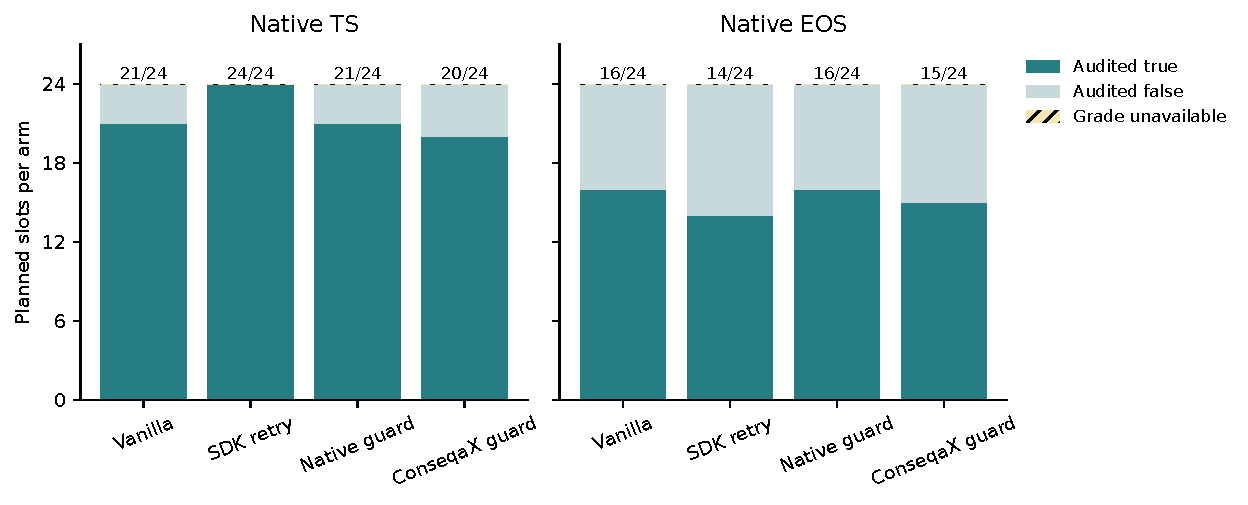
\includegraphics[width=\textwidth,height=0.67\textheight,keepaspectratio]{limbo-outcomes.pdf}
\caption{Native TS/EOS true, false and unavailable grades over all 24 planned slots per arm. Error returns with audited settled grades remain physically assessable.}
\label{fig:limbo-outcomes}
\end{figure*}

\begin{figure*}[t]
\centering
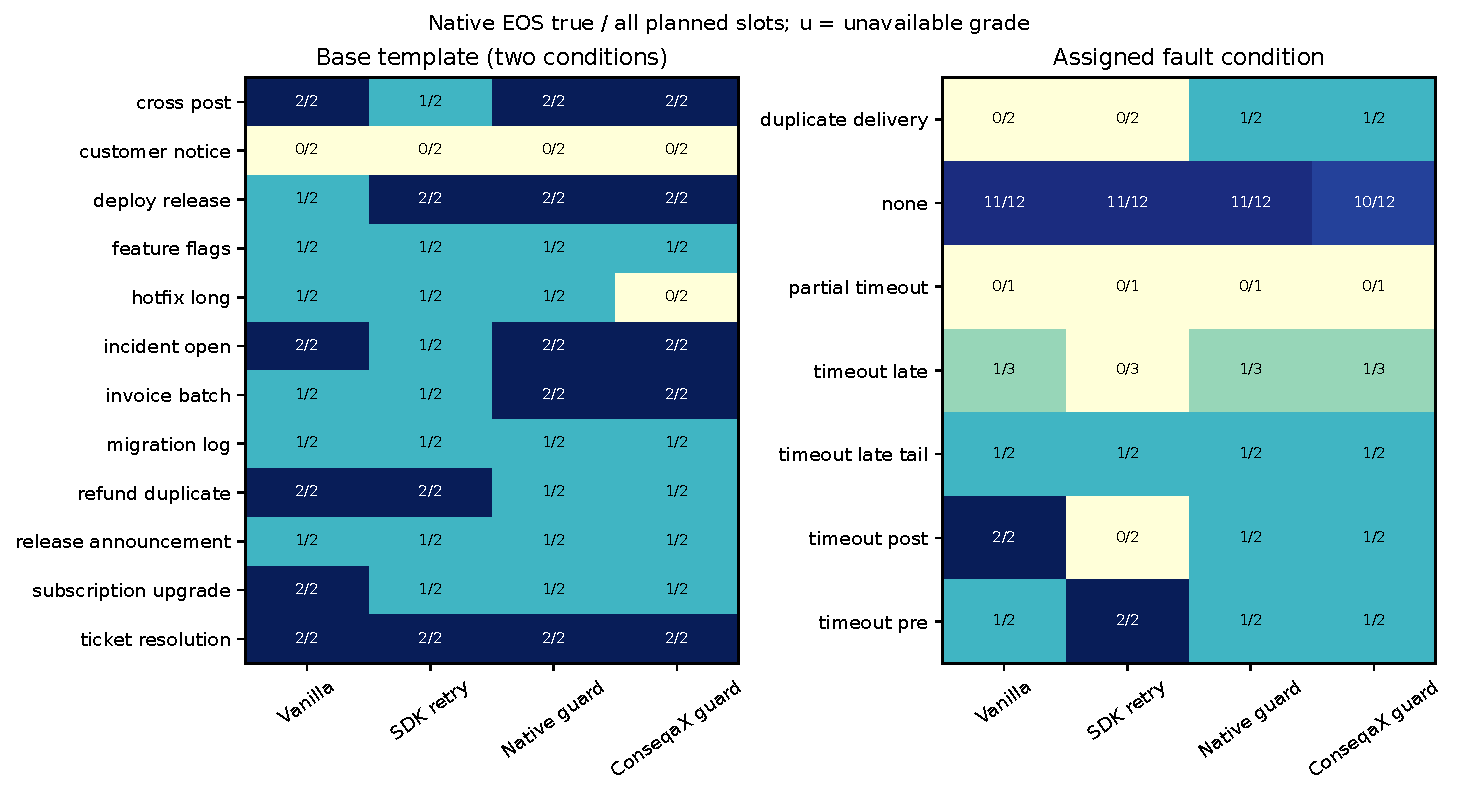
\includegraphics[width=\textwidth,height=0.67\textheight,keepaspectratio]{limbo-stratification.pdf}
\caption{Native EOS true over all planned slots by base template and assigned fault. Unavailable grades remain marked. Strata are finite and descriptive; fault triggering is not an inclusion rule.}
\label{fig:limbo-stratification}
\end{figure*}

\begin{figure*}[t]
\centering
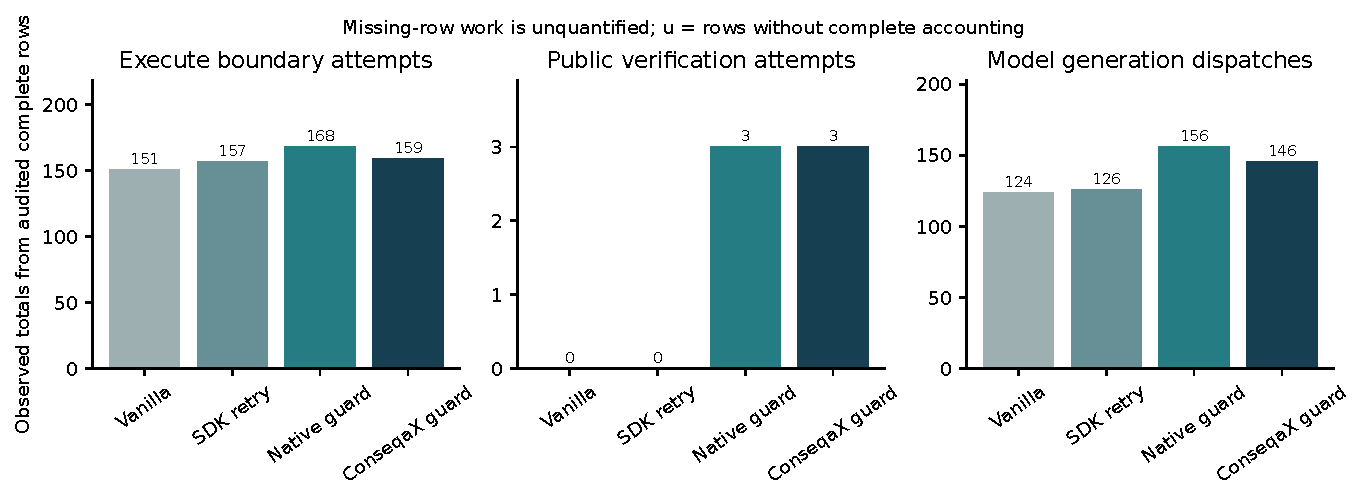
\includegraphics[width=\textwidth,height=0.67\textheight,keepaspectratio]{limbo-costs.pdf}
\caption{Observed execute, public verification and model-dispatch totals from complete audited rows. Missing-row work is unquantified. Boundary attempts are not physical effect counts or isolated SDK overhead.}
\label{fig:limbo-costs}
\end{figure*}
